\documentclass[]{article}


\usepackage[utf8]{inputenc}
\usepackage{hyperref}
\usepackage[acronym]{glossaries}
\usepackage{graphicx}

%--------------------packages fore vhdl stuff----------------------------
\usepackage[T1]{fontenc}
\usepackage{beramono}% monospaced font with bold variant

\usepackage{listings}
\lstdefinelanguage{VHDL}{
	morekeywords={
		library,use,all,entity,is,port,in,out,end,architecture,of,
		begin,and
	},
	morecomment=[l]--
}

\usepackage{xcolor}
\colorlet{keyword}{blue!100!black!80}
\colorlet{comment}{green!90!black!90}
\lstdefinestyle{vhdl}{
	language     = VHDL,
	basicstyle   = \ttfamily,
	keywordstyle = \color{keyword}\bfseries,
	commentstyle = \color{comment}
}

%--------------------todo stuff-----------------------------------------
\usepackage[colorinlistoftodos,prependcaption,textsize=tiny]{todonotes}
%opening
\hypersetup{
	colorlinks,
	citecolor=black,
	filecolor=black,
	linkcolor=black,
	urlcolor=black
}

%---------------------hyper link stuff------------------------------------
\usepackage{hyperref}
\hypersetup{
	colorlinks,
	citecolor=black,
	filecolor=black,
	linkcolor=black,
	urlcolor=black
}

%opening
%-----------------------glossary-------------------------------------------
\makenoidxglossaries % use TeX to sort

%
\loadglsentries{glos_list.tex}
\title{Technical status Zifra card}
\author{Torbjörn}

\begin{document}

\maketitle
\tableofcontents
\newpage
\newpage

\begin{abstract}
This document is meant to clarify what have bin don and what is needed to be don.
\end{abstract}

\newpage


%\section{todo}
%Here i will list stuff i come up whit so that i can write about them later.

%\begin{itemize}
%	\item crypto scheem whit curv 25519
%	\item Alex algorithm
%	\item hiding files in fat
%	\item fat format
%\end{itemize}




\section{Brief description}
We will here shortly describe what the Zifra card is meant to be.
It is an memory card that is supost to protect data by encrypting the data that is writen to it.
This is done whit the help of multiple \gls{keys} and \gls{cipher}.
i
\section{System overview}
We will here describe the way we want the system to work.
Fore the case of explenation we will use an camera as example case.
We will first talk about the key generation secondly encryption and finally about decryption step.

\subsection{Key generation}
There is three type of keys used in the crypto scheme.
The first two keys are pre-generated as an key pair on an safe device one \acrfull{priKey} and one \acrfull{pubKey}. 
The pri\_key is saved fore later use and the pub\_key is transfered and saved on the sd-card see Figure \ref{fig:key_gen}.
Then the user puts the sd card in an camera.
When the camera boots up an random number is generated this is the \acrfull{randKey} this number is then encrypted whit the Pub\_key and saved on the memory.

\begin{figure}[h]
	\centering
	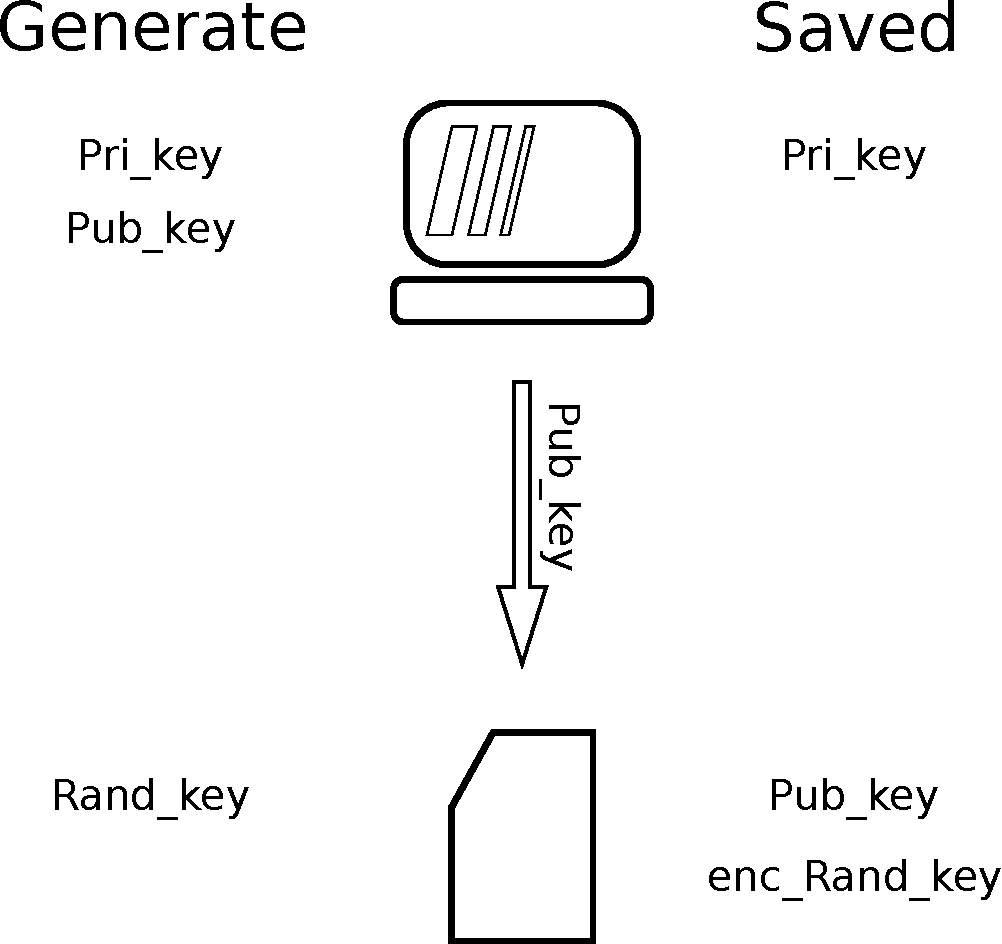
\includegraphics[width=0.8\textwidth]{ilustrations/Key_generations.pdf}
	\caption{This illustration shows where the keys are generated and where they are stored}
	\label{fig:key_gen}
\end{figure}
\clearpage
\newpage
\subsection{Encryption}
The Rand\_key\footnote{This is the non encrypted random key.} is then used as the key input in the chacha cipher to encrypt the data before it is saved to the memory se Figure \ref{fig:encrypt}.
When the system is powered of the Rand\_key that is only stored in the FPGA disappeared due to the nature of an FPGA.
The generation and encryption of the Rand\_key is repeated fore each session.
So there will be multiple enc\_Rand\_key:s stored on the memory one fore each session.

\begin{figure}[h]
	\centering
	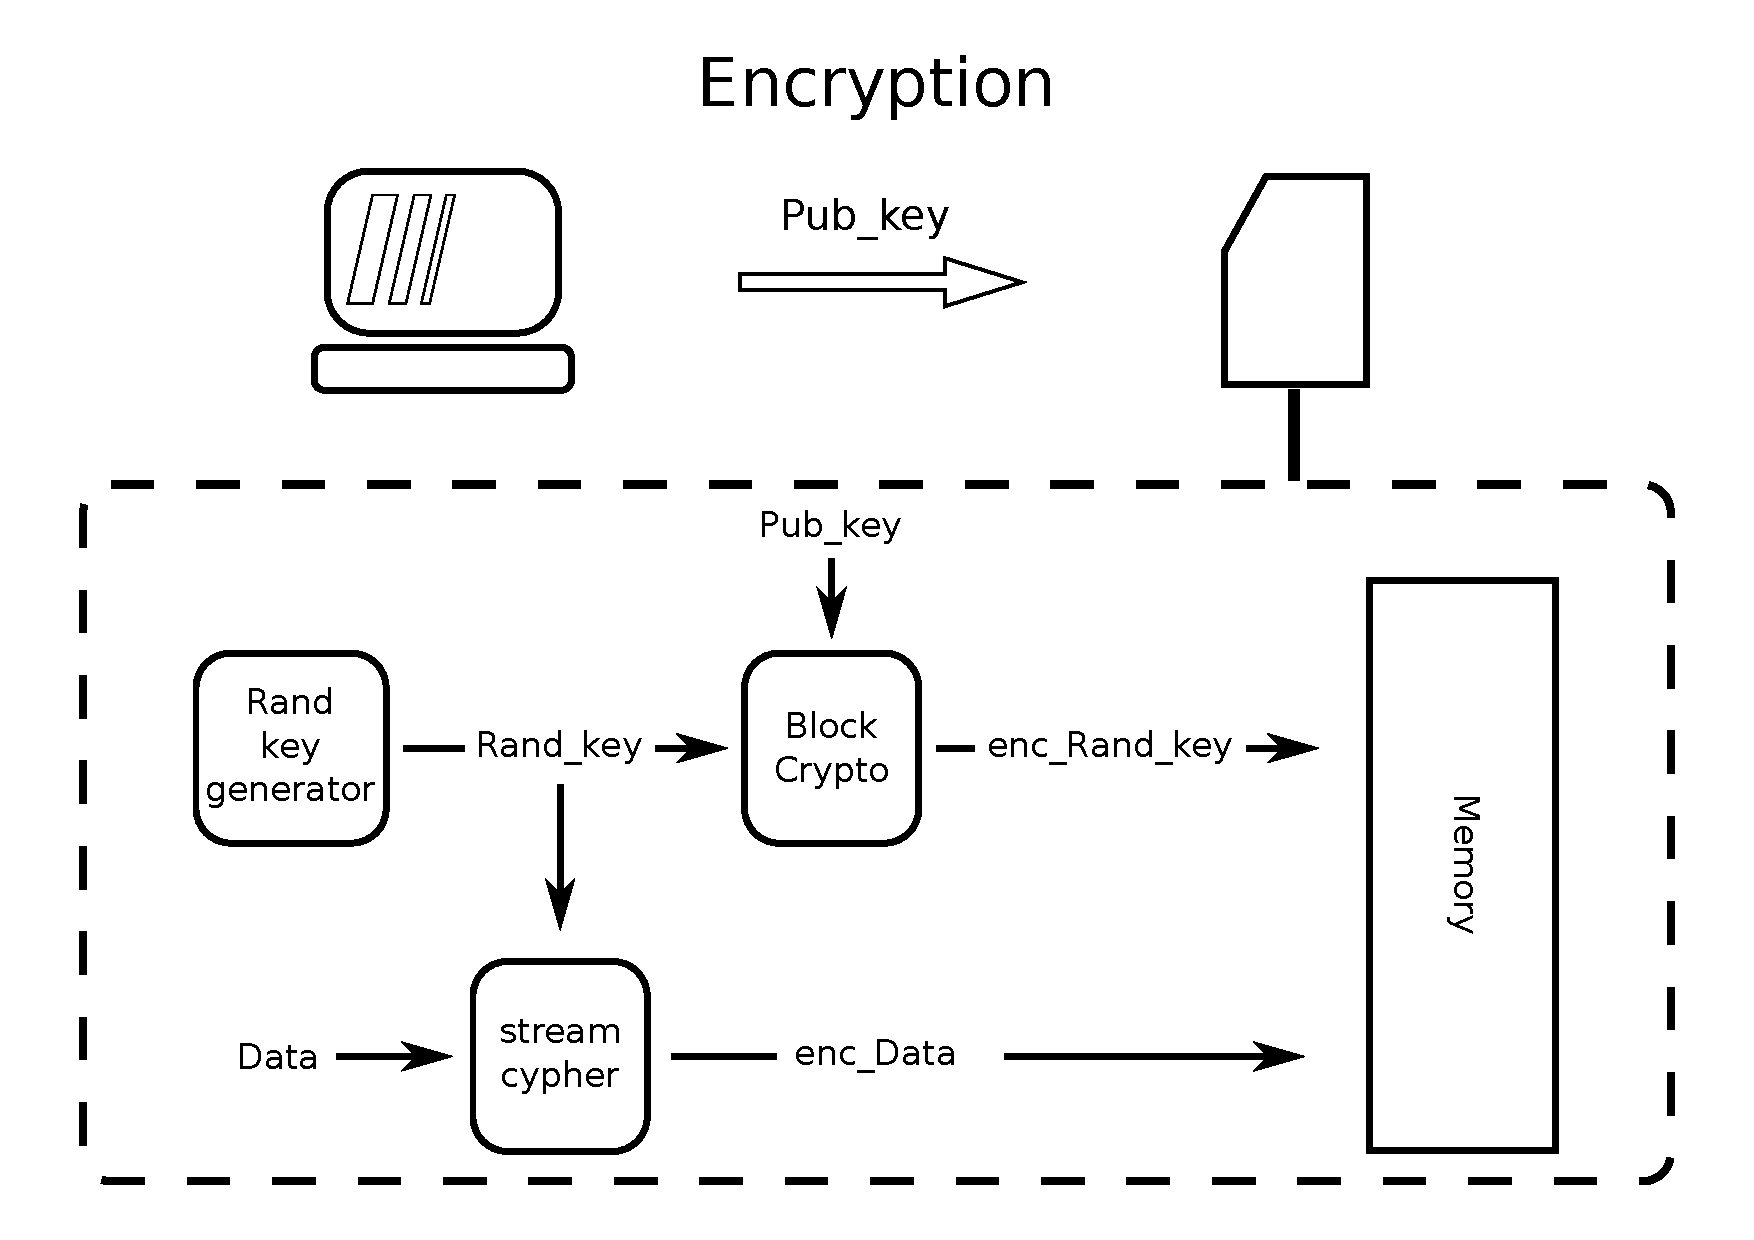
\includegraphics[width=0.8\textwidth]{ilustrations/encryption.pdf}
	\caption{Basic data flow in encryption step}
	\label{fig:encrypt}
\end{figure}
\clearpage
\newpage
\subsection{Decryption}
When decrypting the data one extracts the encrypted data and the \acrfull{encRandKey} on to the safe device were the Pri\_key is saved.
Then we use the Pri\_key to decrypt the enc\_Rand\_key:s and then we can use the Rand\_key:s to decrypt the data se Figure \ref{fig:decrypt}.

\begin{figure}[h]
	\centering
	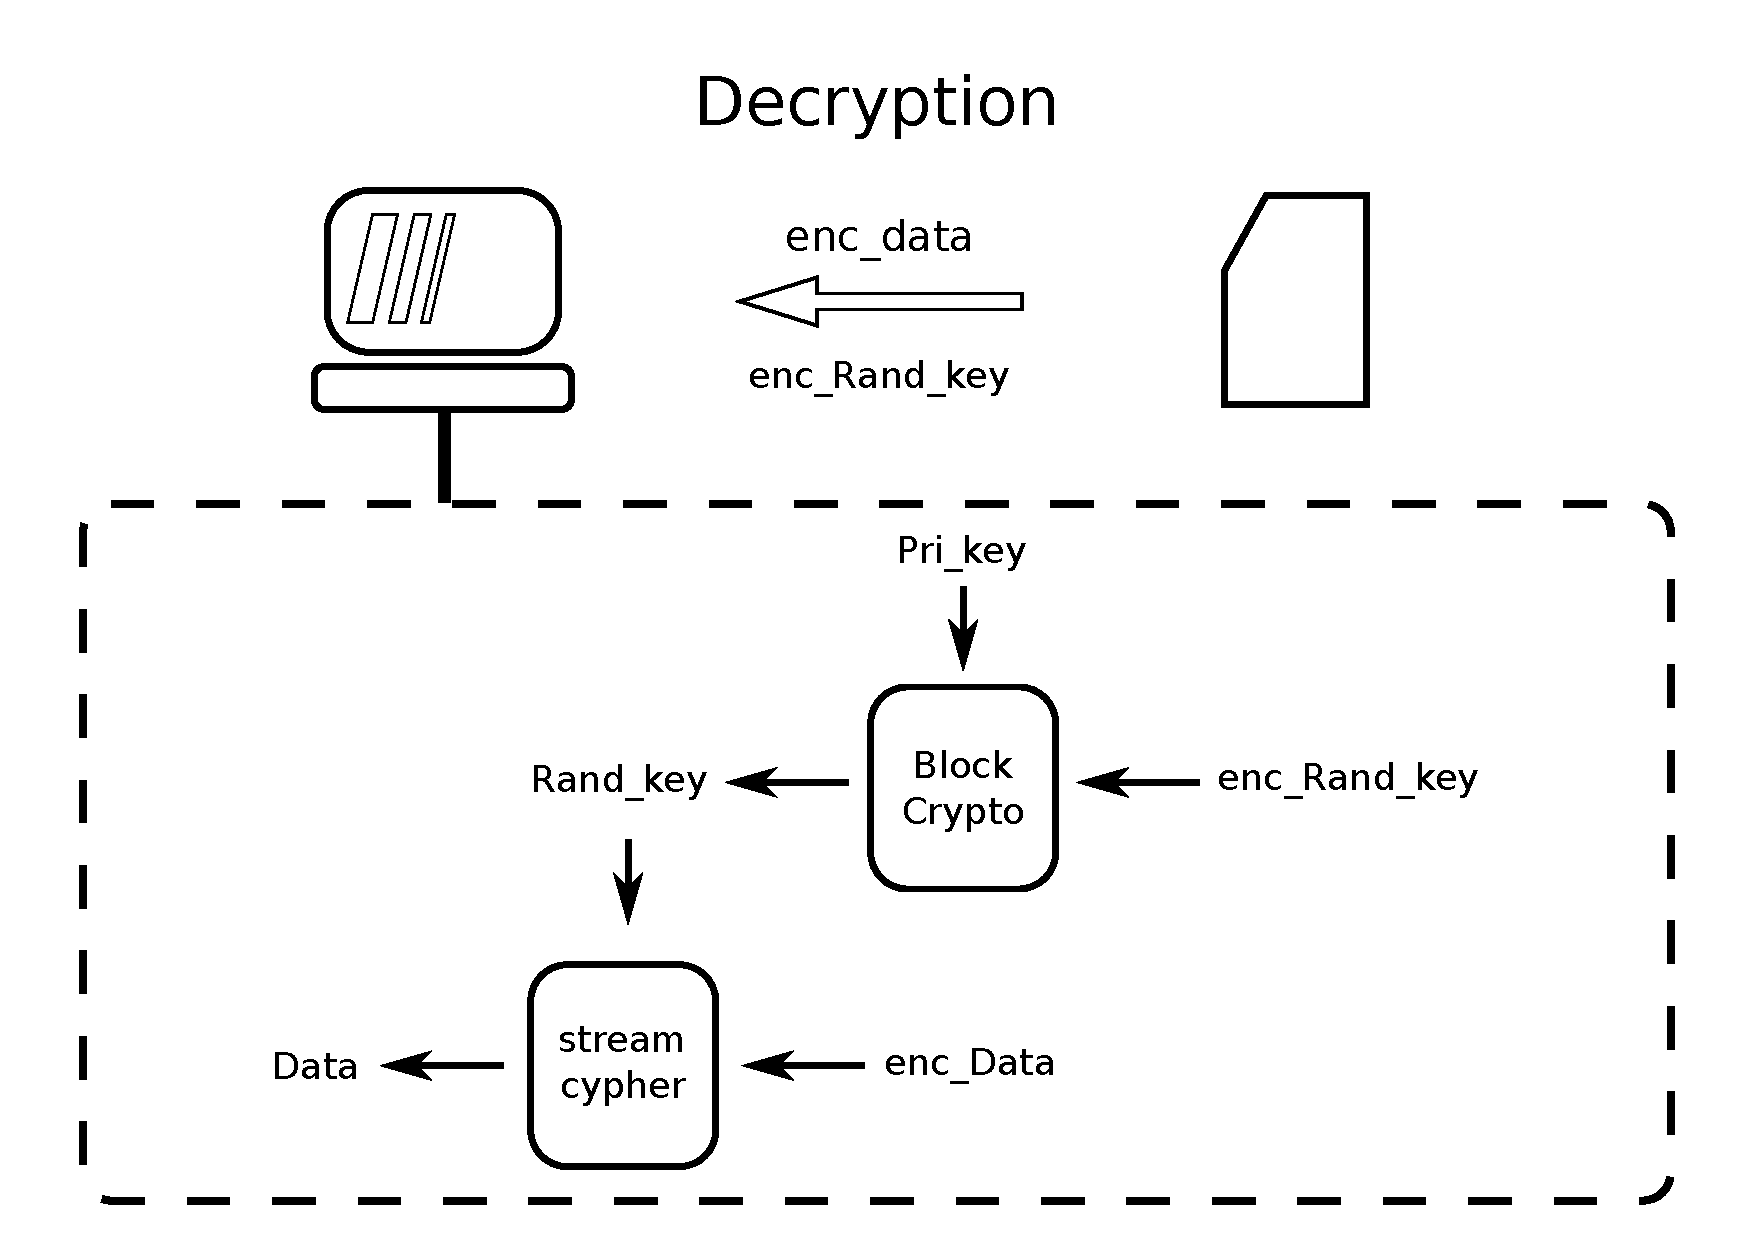
\includegraphics[width=0.8\textwidth]{ilustrations/decryption.pdf}
	\caption{basic data flow in decryption step}
	\label{fig:decrypt}
\end{figure}



\section{Hardware}
The hardware was intended to be an \acrfull{pcb} whit an \acrfull{fpga} whit an memory and some suport component.
The FPGA that we use is the Artix7 t35.


\section{sd slave progress}
The sd slave comes form the Google vault project \cite{GV}.
This part of the project dose not work yet.

We have extracted the blocks that we think are needed fore the project.
There test bench to test and send commands to the design and see what responses the device sends back.
So fare we can read and write from the first sector in the memory but not to any other sector.

\subsection{Development environment}

Here I will state the steps to get the debugging platform working.
The system is designed fore the arty z7 board.

Firs start the Vivado project.
Second we need to sett the board to jtag boot mode this is don whit an jumper on the board.
Follow this whit an power chicle.
Open hardware manager and open target.
Right click on the FPGA to add configuration memory device\footnote{If this dose not work it might mean that you might need to remove an old one, right click on the memory and choose remove}.
\begin{table}
	\centering
	\begin{tabular}{l|r}
		Function		& Setting		\\
		\hline
		Manufacturer	& Spansion  	\\ 
		Settings 		& Value  		\\ 
		Density  		& 256  			\\ 
		Type 			& qspi  		\\ 
		Width 			& x4-single  	
	\end{tabular}
	\caption{This table includes settings fore configuring the memory on the artyz7 board.}
	\label{table:memorySettings}
\end{table}

This produces two results we pick the \emph{3.3V} version and press ok.
Vivado now asks if we want to program it we say ok.
Now we need to pick the \emph{.elf} and \emph{boot.bin} files.
The boot.bin lives in the root of the project. 
And the \emph{fsbl.elf} file resides in \texttt{*.sdk\textbackslash fsbl\textbackslash Debug}.
Then program.
Sett boot jumper to spi mode and power cycle.

Then I used minicom\footnote{minicom is an text based terminal emulator} to connect to the system boudrate 115200.
mmc info shuld give info about the device.
Use \texttt{read mmc 0 0 1} to read first sector and \texttt{write mmc 0 0 1} to write first sector.


\section{chacha}
The stream cipher that was decided to use fore the data encryption ip called chacha \cite{chacha} developed by Joachim Strömbergson \cite{joachim}.  
We have made an axi ip block out of it one stream port fore the data and one address port fore the setting example iv and key se Figure \ref{fig:chacha}.
There is an test bench that show how the axi block is intended to bee used.

\begin{figure}[h]
	\centering
	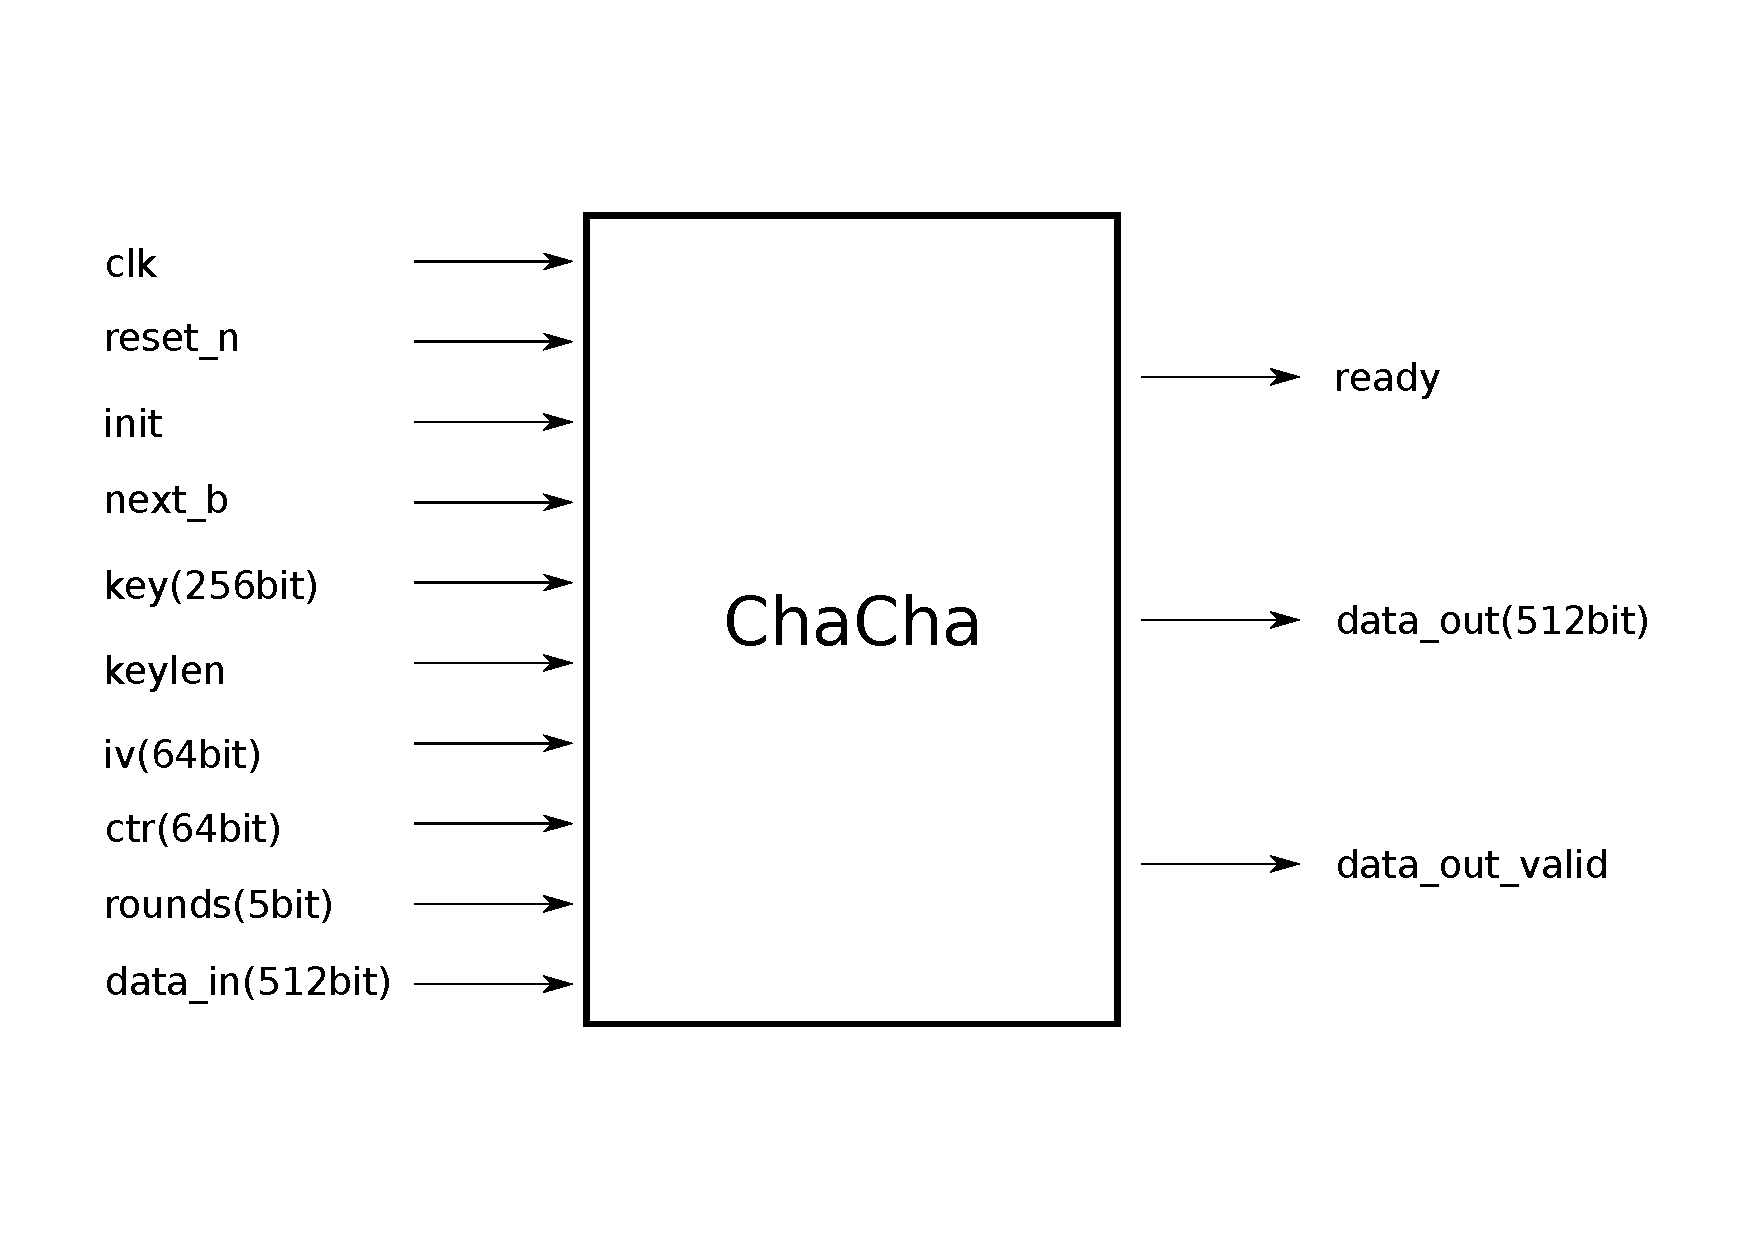
\includegraphics[width=0.8\textwidth]{ilustrations/chacha.pdf}
	\caption{Port configuration chacha cipher}
	\label{fig:chacha}
\end{figure}


\section{Helpful data}
This section will list information that have bin collected during the project that might help further development.

\subsection{CSD list}
During the debugging we listed the CSD values that was used in the \gls{gvsdslave} we also made an list of the other CSD and CID values.
We list the CSD list 1.0, 2.0 and the CID list also the original CSD settings from the Google Vault.

\begin{table}[h]
\centering
\resizebox{\columnwidth}{!}{%
\begin{tabular}{|l|l|l|}
	&This is the list from part1 Version (1.0)& \\
	\hline
	&& \\
	Name &Descripton&CSD-slice \\
	CSD structure&CSD structure&[127:126] \\
	-&reserved&[125:120] \\
	TAAC&data read access-time-1&[119:112] \\
	NSAC&data read access-time-2 in CLK cycles (NSAC * 100)&[111:104] \\
	TRAN\_SPEED&max. read data block length&[103:96] \\
	CCC&card command classes&[95:84] \\
	READ\_BL\_LEN&max. read data block length&[83:80] \\
	READ\_BL\_PARTIAL&partial blocks for read allowed&[79:79] \\
	WRITE\_BLK\_MISALIGN&write block misalignment&[78:78] \\
	READ\_BLK\_MISALIGN&read block misalignment&[77:77] \\
	DSR\_IMP&DSR implemented&[76:76] \\
	-&reserved&[75:74] \\
	C\_SIZE&device size&[73:62] \\
	VDD\_R\_CURR\_MIN&max.read current @ VDD min&[61:59] \\
	VDD\_R\_CURR\_MAX&max.read current @ VDD max&[58:56] \\
	VDD\_W\_CURR\_MIN&max.write current @ VDD min&[55:53] \\
	VDD\_W\_CURR\_MAX&max.write current @ VDD max&[52:50] \\ 
	C\_SIZE\_MULT&device size multiplier&[49:47] \\
	ERASE\_BLK\_EN&erase single block enable&[46:46] \\
	SECTOR\_SIZE&erase sector size&[45:39] \\
	WP\_GRP\_SIZE&write protect group size&[38:32] \\
	WP\_GRP\_ENABLE&write protect proup enable&[31:31] \\
	-&reserved&[30:29] \\
	R2W\_FACTOR&write speed factor&[28:26]  \\
	WRITE\_BL\_LEN&max. write data block length&[25:22] \\
	WRITE\_BL\_PARTIAL&partial blocks for write allowed&[21:21] \\
	-&reserved&[20:16]  \\
	FILE\_FORMAT\_GRP&file format group&[15:15] \\
	COPY&copy flag&[14:14] \\
	PERM\_WRITE\_PROTECT&premanet write protection&[13:13] \\
	TMP\_WRITE\_PROTECT&temporary write protection&[12:12] \\
	FILE\_FORMAT\_GRP&file format&[11:10] \\
	-&reserved&[9:8] \\
	CRC&crc&[7:1] \\
	-&not used always '1'&[0:0] \\
\end{tabular}%
}
\caption{Table shows CSD list Version 1.0}
\label{table:cs12.0}
\end{table}

\begin{table}[h]
\centering
\resizebox{\columnwidth}{!}{%
\begin{tabular}{|l|l|l|}
&This is the list from part1 Version (2.0)& \\
\hline
&& \\
Name &Descripton&CSD-slice \\
CSD structure&CSD structure&[127:126] \\
-&reserved&[125:120] \\
TAAC&data read access-time-1&[119:112] \\
NSAC&data read access-time-2 in CLK cycles (NSAC * 100)&[111:104] \\
TRAN\_SPEED&max. read data block length&[103:96] \\
CCC&card command classes&[95:84] \\
READ\_BL\_LEN&max. read data block length&[83:80] \\
READ\_BL\_PARTIAL&partial blocks for read allowed&[79:79] \\
WRITE\_BLK\_MISALIGN&write block misalignment&[78:78] \\
READ\_BLKe\_MISALIGN&read block misalignment&[77:77] \\
DSR\_IMP&DSR implemented&[76:76] \\
-&reserved&[75:70] \\
C\_SIZE&device size&[69:48] \\
&reserved&[47:47] \\
ERASE\_BLK\_EN&erase single block enable&[46:46] \\
SECTOR\_SIZE&erase sector size&[45:39] \\
WP\_GRP\_SIZE&write protect group size&[38:32] \\
WP\_GRP\_ENABLE&write protect proup enable&[31:31] \\
-&reserved&[30:29] \\
R2W\_FACTOR&write speed factor&[28:26]  \\
WRITE\_BL\_LEN&max. write data block length&[25:22] \\
WRITE\_BL\_PARTIAL&partial blocks for write allowed&[21:21] \\
-&reserved&[20:16]  \\
FILE\_FORMAT\_GRP&file format group&[15:15] \\
COPY&copy flag&[14:14] \\
PERM\_WRITE\_PROTECT&premanet write protection&[13:13] \\
TMP\_WRITE\_PROTECT&temporary write protection&[12:12] \\
FILE\_FORMAT\_GRP&file format&[11:10] \\
-&reserved&[9:8] \\
CRC&crc&[7:1] \\
-&not used always '1'&[0:0] \\
\end{tabular}%
}
\caption{Table shows CSD list Version 2.0}
\label{table:csd2.0}
\end{table}


\begin{table}[h]
\centering
\resizebox{\columnwidth}{!}{%
\begin{tabular}{l|l|l|l}
	&Settings from GV sd\_parms.vh&& \\
	\hline
	&&& \\
	Name&Value&&Comment \\
	CSD\_CSD\_STRUCTURE&b01&& \\
	CSD\_TAAC&h0E&& \\
	CSD\_NSAC&h00&& \\
	CSD\_TRAN\_SPEED\_25&h32&& \\
	CSD\_TRAN\_SPEED\_50&h5A&& \\
	CSD\_CCC&b01\_1\_110110101&& \\
	CSD\_READ\_BL\_LEN&9&&512 byte Blocks \\
	CSD\_READ\_BL\_PARTIAL&h0&&Partial block reads not implemented \\
	CSD\_WRITE\_BLK\_MISALIGN&h0&&Write misalingned block not implemented \\
	CSD\_READ\_BLK\_MISALIGN&h0&&Read misaligned block not implemented \\
	CSD\_DSR\_IMPL&h0&&DSR not implemented \\
	CSD\_C\_SIZE&8&&4.5 MBYTE \\
	SD\_TOTAL\_BLOCKS&(CSD\_C\_SIZE+1) * 1024&9216& \\
	CSD\_ERASE\_BLK\_EN&h1&& \\
	CSD\_SECTOR\_SIZE&h7F&& \\
	CSD\_WP\_GRP\_SIZE&h0&& \\
	CSD\_WP\_GRP\_ENABLE&h0&& \\
	CSD\_R2W\_FACTOR&b010&& \\
	CSD\_WRITE\_BL\_LEN&h9&& \\
	CSD\_WRITE\_BL\_PARTIAL&h0&& \\
	CSD\_FILE\_FORMAT\_GRP&h0&& \\
	CSD\_COPY&h0&& \\
	CSD\_PERM\_WRITE\_PROTECT&h0&& \\
	CSD\_TMP\_WRITE\_PROTECT&h0&& \\
	CSD\_FILE\_FORMAT&b00&& \\
	&&& \\
	&&& \\
	&Settings from GV sd\_const.vh&& \\
	&&& \\
	Name&Value&& \\
	CMD9\_SEND\_CSD&d9&& \\
	CMD27\_PROGRAM\_CSD&d27&& \\
	STAT\_CSD\_OVERWRITE&d16&& \\
\end{tabular}%
}
\caption{This is the CSD settings that was originally in the Google Vault project. }
\label{table:gvCsd}
\end{table}

\begin{table}[h]
	\centering
	\resizebox{\columnwidth}{!}{%
	\begin{tabular}{l|l|l|l}
		
	Name&Field &Width&CID-slice \\
	\hline
	&&& \\
	Manufactire ID&MID&8&[127:120] \\
	OEM/Application ID&OID&16&[119:104] \\
	Product name&PNM&40&[103:64] \\
	Prodict revision&PRV&8&[63:56] \\
	Product serial number&PSN&32&[55:24] \\
	reserved&--&4&[23:20] \\
	Manufacturing date&MDT&12&[19:8] \\
	CRC7 checksum&CRC&7&[7:1] \\
	"not used, always 1"&-&1&[0:0] 
		
	\end{tabular}%
	}
	\caption{This table shows the CID list}
	\label{table:cidList}
\end{table}

\clearpage

\section{Whishlist}
Here we will list some features that we wold like to have in the future.
Thees are extras but good to have.

\subsection{Hidden files}
We wold like to have the possibility to hide the files so that every time you start up the memory card it looks empty.
This wold be don by making an temporary FAT table that is used during the session then hidden between the \gls{mbs} and the real FAT table.

\subsection{See pictures when camera is still on}
We wold like to be able to look at the pictures during the session.
This wold mean that the cipher needs to work in both directions during the session.

\subsection{Fake pictures}
We wold also like to be able to prep the memory card whit fake data in the camera case that wold be preloaded whit pictures.
Thees wold show up if someone wold inspect the card.
This wold also be helped by the see pictures while session is active if the system is tested.




\clearpage
\newpage
\printglossary[type=\acronymtype]
\printnoidxglossaries


\bibliography{mybib}{}
\bibliographystyle{plain}
\end{document}

 












